\documentclass[a4paper,12pt,titlepage]{article}
\usepackage[utf8]{inputenc}
\usepackage{graphicx} % Required for inserting images
\usepackage[spanish,es-tabla]{babel}
\usepackage[none]{hyphenat}
\usepackage[justification=centering]{caption}
\usepackage{subcaption}
\usepackage{amssymb, amsmath}
\usepackage{gensymb}
\usepackage{fancyhdr}
\usepackage{wrapfig}


\lhead{Momento de inercia}
\rhead{Gonzalo Bastos González}

\pagestyle{fancy}

\title{Momento de inercia}
\author{Gonzalo Bastos González}

\begin{document}

\maketitle
\tableofcontents

\newpage

\section{Objetivos e introducción teórica}

Esta práctica gira alrededor del concepto de momento de inercia y tiene dos objetivos principales:

\begin{itemize}
    \item Medir experimentalmente el momento de inercia de diferentes cuerpos
    \item Verificar el teorema de Steiner
\end{itemize}

Para comenzar con nuestra práctica en primer necesitamos unas bases teóricas sobre las que realizar nuestros experimentos. La práctica parte del concepto de momento de inercia, magnitud que se define como la cuantificación de la inercia de rotación de un cuerpo. Matemáticamente el concepto de momento de inercia de un sistema de partículas se define como:

\begin{equation}
    I = \sum_i^N m_i r_i^2
\end{equation}

Esta fórmula puede generalizara para cuerpos de masa continua, que son con los que trabajamos, con la siguiente expresión:

\begin{equation}
    I = \int r^2 dm
    \label{Def MI}
\end{equation}

Si aplicamos esta expresión a determinados cuerpos geómetricos simples podemos obtener una expresión simplificada para su momento de inercia respecto a su eje de simetría:

\begin{equation}
    \begin{gathered}
        \text{Disco: } I=\frac{MR^2}{2} \\
        \text{Cilindro: } I = \frac{MR^2}{2}\\
        \text{Esfera: } I = \frac{2MR^2}{5} \\
        \text{Barra: } I = \frac{ML^2}{12}
        \label{MI cuerpos geometricos}
    \end{gathered}
\end{equation}

Siendo $M$ la masa del cuerpo, $R$ su radio y $L$ su longitud.
\par A partir de la definición de momento de inercia podemos intuir que esta magnitud va a presentar una gran relación con la rotación de los cuerpos y, por tanto, las magnitudes que la definen. Partiremos de la ecuación fundamental del movimiento de rotación:

\begin{equation}
    \vec{M} = \frac{d\vec{L}}{dt}
\end{equation}

Donde se relaciona el momento de la fuerza que produce la rotación ($\vec{M}=\vec{R}\times \vec{F}$) con la derivada del momento angular $\vec{L}$. En un sólido rígido el momento angular se puede expresar como:

\begin{equation}
    \vec{L} = I \vec{\omega}
\end{equation}

Siendo $\vec{\omega}$ la velocidad angular. Cuando el giro se produce sobre uno de los ejes principales del cuerpo el momento angular tiene la misma dirección que $\vec{\omega}$ y podemos emplear la expresión anterior en módulos ($L=I_e\omega$).

\par Para nuestra práctica mediremos el momento de inercia respecto a un eje a partir del período de oscilación de su rotación cuando se le hace girar sometido a la fuerza recuperadora de un resorte elástico. El momento de esa fuerza recuperadora cumple la siguiente relación:

\begin{equation}
    M = -D\varphi
    \label{Constante resorte}
\end{equation}

Donde $D$ es una constante propia del resorte y $\varphi$ es el ángulo girado. A partir de esta ecuación vamos a buscar una relación que nos permita calcular el momento de inercia del cuerpo respecto al eje a partir del momento de la fuerza, que podremos determinar experimentalmente:

\begin{equation}
    M = \frac{dL}{dt};\; L=I\omega;\; \omega = \frac{d\varphi}{dt} \Rightarrow M = I \frac{d^2\varphi}{dt^2}
\end{equation}

Teniendo en cuenta la expresión anterior y la Ec.\ref{Constante resorte} obtenemos la siguiente expresión:

\begin{equation}
    \frac{d^2\varphi}{dt^2} = -\frac{D}{I}\varphi
\end{equation}

Esta es la ecuación diferencial que describe el comportamiento de un oscilador simple, si la resolvemos obtenemos la siguiente expresión que nos ayuda a modelizar la oscilación:

\begin{equation}
    \varphi(t) = \varphi_0 \cos\left (\sqrt{\frac{D}{I}}t+\phi_0\right ) 
\end{equation}

El período de este movimiento armónico viene dado por la siguiente expresión:

\begin{equation}
    T = 2\pi\sqrt{\frac{I}{D}}
    \label{Periodo oscilacion}
\end{equation}


Esta expresión nos permitirá calcular el momento de inercia de nuestro cuerpo midiendo su período de oscilación cuando se somete a la fuerza recuperadora del resorte, algo mucho más fácil de medir experimentalmente. Esta igualdad nos servirá como fundamento para calcular todos los momentos de inercia medidos a lo largo de toda la práctica.

\par La segunda parte de la práctica se centra en verificar el teorema de Steiner, que afirma que el momento de inercia de un sólido rígido respecto a un eje es igual al momento de inercia respecto a otro eje paralelo que pasa por el centro de masas, más el producto de la masa del sólido por la distancia que separa ambos ejes al cuadrado. Matemáticamente se puede expresar como:

\begin{equation}
    I_{ee} = I_0 + md^2
    \label{Steiner}
\end{equation}

\section{Materiales y metodología}

Los materiales empleados para el estudio de sus propiedades fueron:

\begin{itemize}
    \item Disco perforado, de $381,39 \;g$ de masa y $29,9 \; cm$ de diámetro.
    \item Esfera maciza, de $659,23 \; g$ de masa y $13,8 \; cm$ de diámetro
    \item Cilindro macizo, de $384,29 \; cm $ de masa y $10 \; cm$ de diámetro
    \item Barra rígida, de $65,7 \; cm$ de longitud
\end{itemize}
La incertidumbre de las medidas masas viene dada por la precisión instrumental de la balanza:
\begin{equation}
    s(m) = 0,01 \; g
\end{equation}
Por otro lado, la incertidumbre de las medidas realizadas con la regla de los diámetros y la longitud de la barra viene dada por la precisión instrumental de la regla empleada:
\begin{equation}
    s(x) = 0,001 \;m
\end{equation}
Para realizar las medidas contamos con los siguientes instrumentos:

\begin{itemize}
    \item Balanza, con una precisión de 0,01 g
    \item Recta milimetrada, con una precisión de 0,001 m
    \item Soporte giratorio dotado de un resorte
    \item Detector fotoeléctrico empleado para medir semiperíodos
    \item Dinamómetro
\end{itemize}

En la siguiente figura podemos ver los materiales empleados:

\begin{figure}[h!]
    \centering
    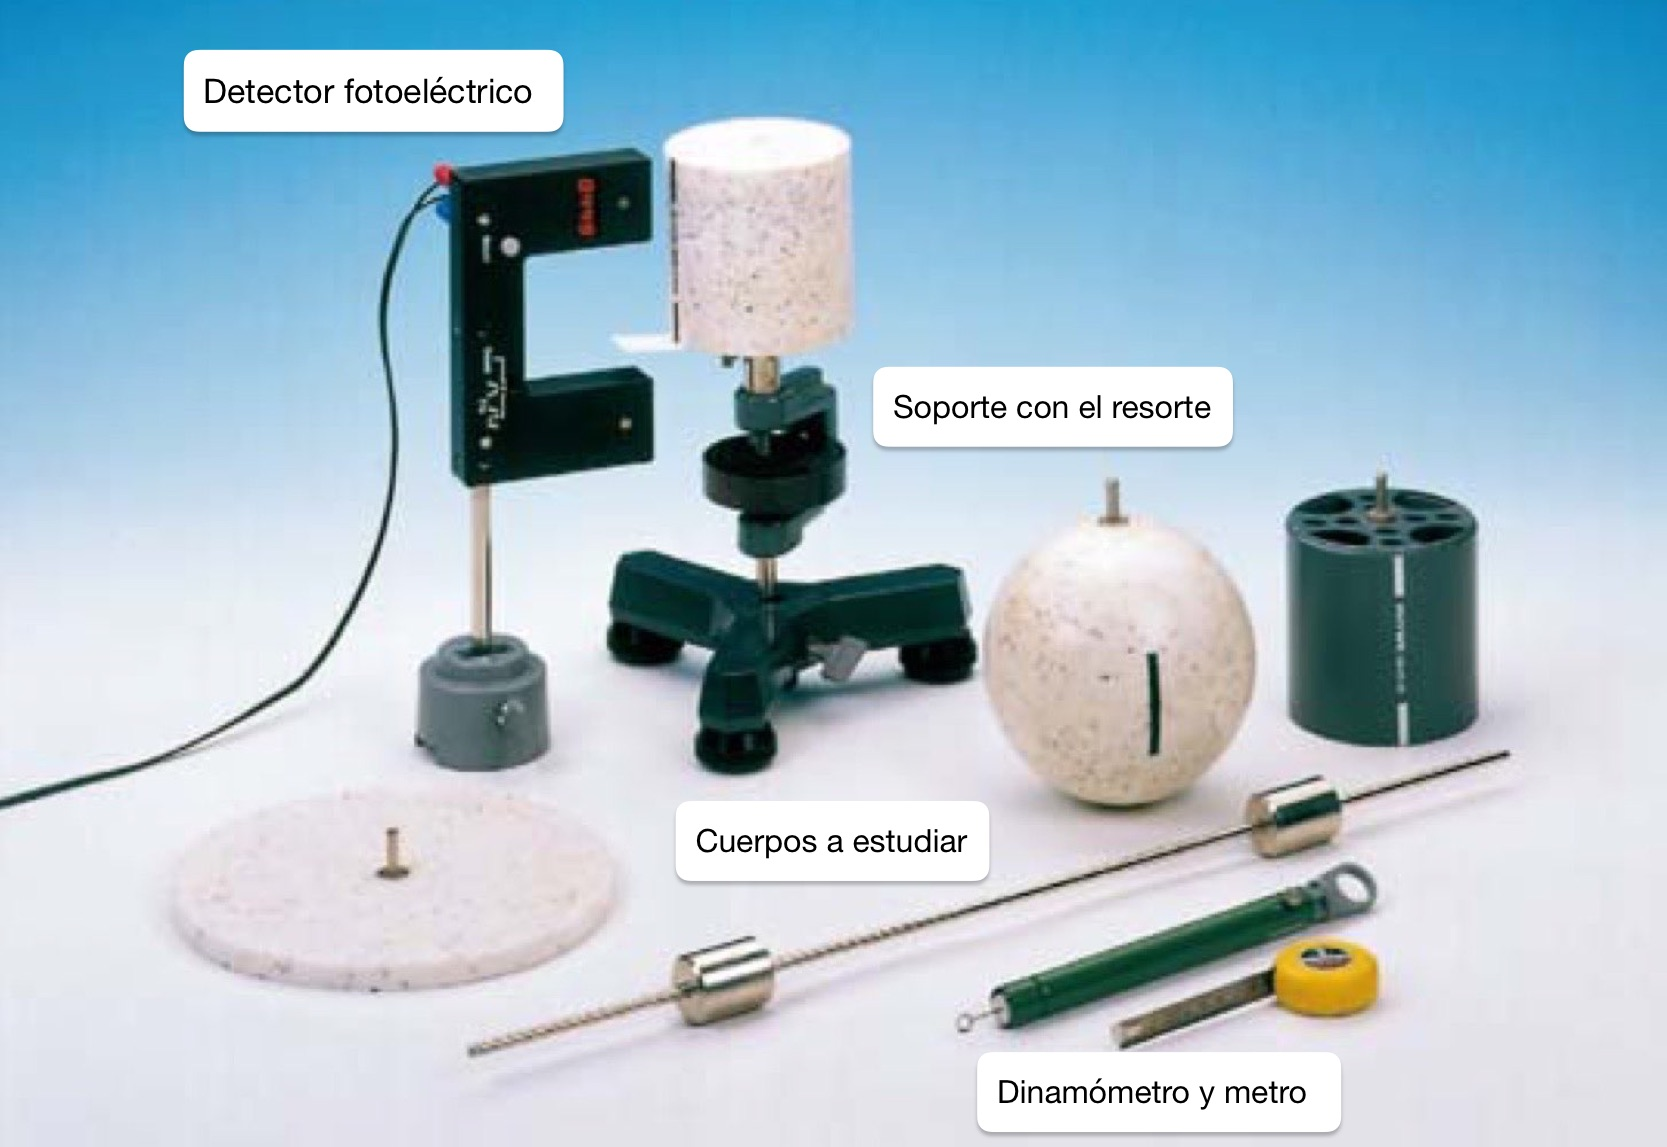
\includegraphics[width=0.75\linewidth]{Images/Material MI-1.jpg}
    \caption{Materiales empleados}
\end{figure}

El procedimiento experimental seguido en cada una de las dos partes de la práctica se detallará a continuación:

\subsection{Determinación del momento de inercia de diferentes cuerpos}

Esta primera parte de la práctica se centra en determinar los momentos de inercia de diferentes cuerpos respecto a su eje de simetría. Para ello aplicaremos la Ec.\ref{Periodo oscilacion}, que relaciona el momento de inercia del cuerpo con su período de oscilación. No obstante, por comodidad a la hora de trabajar con el detector fotoeléctrico hemos decidido trabajar con semiperíodos. Por tanto la expresión de la Ec.\ref{Periodo oscilacion} se transforma en:

\begin{equation}
    T_{1/2} = \pi \sqrt{\frac{I}{D}}
    \label{SemiT osc}
\end{equation}

Como observamos en la expresión anterior la relación entre el semiperíodo y el momento de inercia depende también de la constante $D$ del resorte, \textit{a priori} desconocida. Para calcular el valor de esa constante partiremos de la Ec.\ref{Constante resorte} ($M=-D\varphi$R) y realizaremos un ajuste por mínimos cuadrados de $M$ frente s $\varphi$, donde la pendiente de la recta será la constante $D$. Para el ajuste tomaremos diez medidas con el dinámometro de la fuerza que es necesario ejercer para rotar el disco un determinado ángulo y, previo cálculo del momento de esas fuerzas, calcularemos la constante.

\par Para calcular los momentos de las fuerzas ejercidas vamos a suponer que el vector fuerza y el vector posición son perpendiculares, lo que nos permitirá trabajar solo con los módulos:

\begin{equation}
    M=RF
\end{equation}

Para la incertidumbre del momento aplicaremos propagación de incertidumbres:

\begin{equation}
    s(M) = \sqrt{F^2s^2(R)+R^2s^2(F)}
\end{equation}

Las incertidumbres involucradas son:

\begin{itemize}
    \item La incertidumbre de la fuerza aplicada, que viene dada por la precisión instrumental del dinamómetro:
    \begin{equation}
        s(F) = 0,01 \; N
    \end{equation}
    \item La incertidumbre del módulo del vector posición, que equivale al radio del disco. Este radio se obtuvo de forma indirecta, midiendo el diámetro del disco con la regla milimetrada que cuenta con una precisión instrumental de 1mm:
    \begin{equation}
        s(R) = \frac{s(d)}{2} = 0,0005 \; m
    \end{equation}
\end{itemize}

Las incertidumbre de los ángulos medidos viene dada por la precisión instrumental del disco:

\begin{equation}
    s(\varphi) = 5^\circ = 0,087 \;rad
\end{equation}

Una vez conocida la constantee $D$ del resorte podemos proceder a estudiar el semiperíodo de rotación bajo el efecto de la fuerza recuperadora del resorte. Para ello, como hemos mencioando anteriormente, mediremos varios valores del semiperíodo empleando el detector fotoeléctrico para poder tener una mejor estimación de su valor. Una vez tengamos nuestro valor de referencia del semiperíodo podremos aplicar la Ec.\ref{SemiT osc} para calcular el momento de inercia de cada cuerpo. En concreto la expresión empleada será:

\begin{equation}
    I = D \left (\frac{T_{1/2}}{\pi}\right )^2
    \label{Calculo MI figuras}
\end{equation}

A partir de propagación de incertidumbres podemos calcular la incertidumbre del momento de inercia experimental:

\begin{equation}
    \begin{gathered}
        s(I) = \sqrt{\left (\frac{\partial I}{\partial D}\right )^2s^2(D) + \left (\frac{\partial I}{\partial T_{1/2}}\right )^2s^2(T_{1/2})}\\
        s(I) = \sqrt{\left (\frac{T_{1/2}}{\pi}\right )^4s^2(D) + \left (\frac{2T_{1/2}D}{\pi^2}\right )^2s^2(T_{1/2})}
        \label{Inc MI figuras}
    \end{gathered}
\end{equation}

Las incertidumbres que participan en esta expresión son:

\begin{itemize}
    \item La incertidumbre de la constante $D$ del resorte, que la obtendremos a partir del ajuste por mínimos cuadrados mencionado anteriormente.
    \item La incertidumbre del semiperíodo de rotación, que viene dada por la precisión instrumental del detector fotoeléctrico:
    \begin{equation}
        s(T_{1/2}) = 0,001 \;s
    \end{equation}
\end{itemize}

Una vez calculados los momentos de inercia experimentales de cada cuerpo debemos compararlos con el valor teórico, calculado a partir de la Ec.\ref{MI cuerpos geometricos} para cada figura concreta. Estos valores teóricos también cuentan con una incertidumbre asociada, pues se calculan en función de las dimensiones de la figura, medidas con la regla milimetrada, y de la masa, medida con la balanza. A continuación detallaremos cuál será la incertidumbre del momento de inercia de cada figura con la que trabajamos, calculadas a partir de propagación de incertidumbres:

\begin{itemize}
    \item El momento de inercia del disco es $\frac{MR^2}{2}$, siendo $M$ su masa y $R$ su radio, por lo que el valor teórico con su incertidumbre es:
    \begin{equation}
        \begin{gathered}
            I_D = 0.004262 \; kg \cdot m^2\\
            s(I_D) = \sqrt{\left (\frac{\partial I_D}{\partial M}\right )^2s^2(M) + \left (\frac{\partial I_D}{\partial R}\right )^2s^2(R)} \\ s(I_D)= \sqrt{\left (\frac{R^2}{2}\right )^2s^2(M) + (MR)^2s^2(R)} = 0.000074 \;kg\cdot m^2
        \end{gathered}
    \end{equation}
    \item El momento de inercia del cilindro tiene la misma ecuación ($\frac{MR^2}{2}$), por lo que aplicando la ecuación anterior con las dimensiones del cilindro obtenemos su momento de inercia con la incertidumbre asociada:
    \begin{equation}
        \begin{gathered}
            I_C = 0.00048036 \; kg \cdot m^2\\
            s(I_C) = 0.00000025 \; kg \cdot m^2
        \end{gathered}
    \end{equation}
    \item El último cuerpo con el que trabajamos en esta parte de la práctica fue la esfera, cuyo momento de inercia es $\frac{2MR^2}{5}$, por lo que el valor teórico con su incertidumbre asociada es de:
    \begin{equation}
        \begin{gathered}
            I_E = 0.000726 \; kg \cdot m^2 \\
            s(I_E) = \sqrt{\left (\frac{2R^2}{5}\right )^2s^2(M) + \left (\frac{4MR}{5}\right )^2s^2(R)} = 0,000045 \; kg\cdot m^2
        \end{gathered}
    \end{equation}
\end{itemize}

\subsection{Verificación del teorema de Steiner}

En esta segunda parte de la práctica trataremos de verificar el teorema de Steiner (Ec.\ref{Steiner}). Para ello estudiaremos el momento de inercia respecto a varios ejes de dos cuerpos, el disco perforado y la varilla metálico. El disco perforado era el del apartado anterior, por lo que sus dimensiones son las mismas. La barra metálica tiene un longitud de $65,7$ cm de longitud y una masa de ?????????????0,14410?????????.

\par Para verficar la igualdad del teorema vamos a realizar una regresión lineal de $I$ frente a $d^2$, la pendiente de esa recta será la masa $m$ del cuerpo y el término independiente será $I_0$. Para ello mediremos diez valores del semiperíodo (Para calcular $I$) con los cuerpos rotando alrededor de varios ejes. En primer lugar mediremos 10 semiperíodos con el cuerpo rotando sobre el eje por el que pasa por el centro de masas para calcular $I_0$. Luego realizaremos este mismo procedimiento con el cuerpo rotando sobre ejes situados a una distancia $d$ del eje paralelo que pasa por el centro de masas.

\par En el caso del disco perforado tomaremos 4 conjuntos de medidas, fijando el disco sobre cada una de las perforaciones, que se sitúan a distancias de 3, 6, 9 y 12 cm del centro de masas respectivamente, como se puede ver en la siguiente figura.

\begin{figure}[h!]
    \centering
    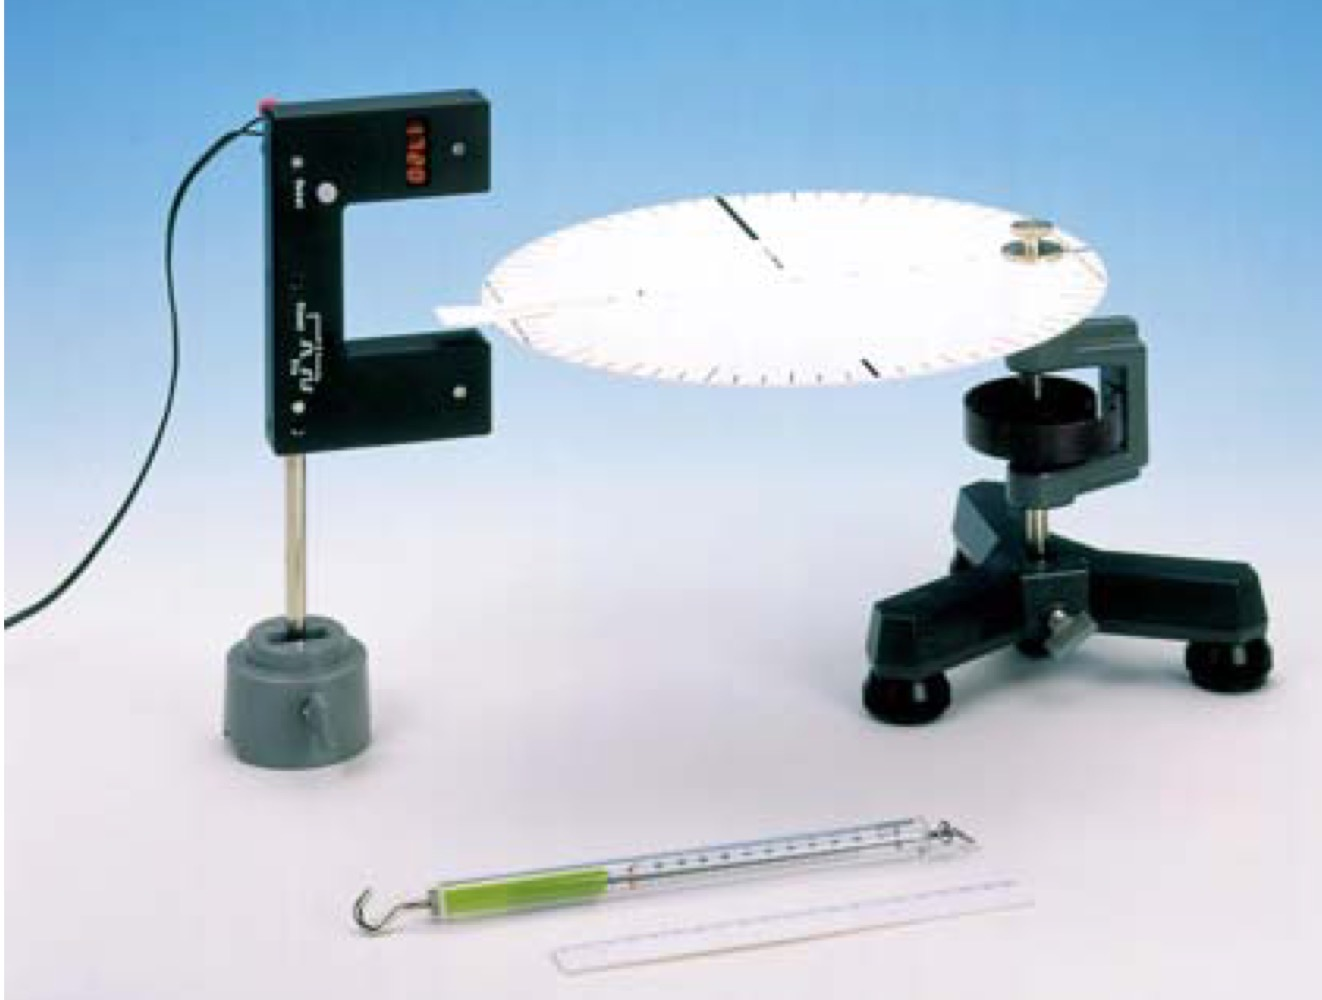
\includegraphics[width=0.65\linewidth]{Images/Material MI 2.jpeg}
    \caption{Montaje experimental para verificar el teorema de Steiner con el disco}
\end{figure}

\par En el caso de la varilla tomaremos 10 conjuntos de medidas, fijando la varilla sobre cada una de las perforaciones transversales con las que cuenta la varilla, situadas a 1 cm la una de la otra. Por tanto las distancias irán de 1 a 10 cm, aumentando de uno en uno. Cabe destacar que en esta parte de la práctica solo pudimos tomar 5 medidas del semiperíodo para cada valor de distancia por problemas técnicos. El problema observado fue que los valores medidos de los semiperíodos no resultaban nada fiables, oscilaban con frecuencia y en muchos momentos perdían la linealidad, por lo que es posible que los resultados en esta parte de la práctica no sean los esperados.

\section{Análisis de datos}

\subsection{Determinación del momento de inercia de diferentes cuerpos}

En la siguiente tabla podemos ver representadas las medidas tomadas en el laboratorio de los ángulo de rotación del disco y las fuerzas, con sus momentos asociados (Teniendo en cuenta que el radio del disco es $14,95 \; cm$), necesarias para producir esas rotaciones:

\begin{table}[h!]
    \centering
    \begin{tabular}{|c|c|c|c|c|c|}
    \hline
    Medida & $F \; (N)$ & $\varphi \; (^{\circ})$ & $\varphi \; (rad)$ & $M \; (N\cdot m)$ & $s(M) \; (N\cdot m)$ \\ \hline
    1  & 0,19 & 90  & 1,571 & 0,0284 & 0,0015 \\ \hline
    2  & 0,23 & 100 & 1,745 & 0,0344 & 0,0015 \\ \hline
    3  & 0,24 & 105 & 1,833 & 0,0359 & 0,0015 \\ \hline
    4  & 0,25 & 115 & 2,007 & 0,0374 & 0,0015 \\ \hline
    5  & 0,27 & 120 & 2,094 & 0,0404 & 0,0015 \\ \hline
    6  & 0,29 & 130 & 2,269 & 0,0434 & 0,0015 \\ \hline
    7  & 0,31 & 145 & 2,531 & 0,0463 & 0,0015 \\ \hline
    8  & 0,33 & 160 & 2,793 & 0,0493 & 0,0015 \\ \hline
    9  & 0,34 & 165 & 2,880 & 0,0508 & 0,0015 \\ \hline
    10 & 0,4  & 180 & 3,142 & 0,0598 & 0,0015 \\ \hline
    \end{tabular}
    \caption{Datos empleados para calcular la constante del resorte}
    \label{Tabla D resorte}
\end{table}

A partir de estos datos vamos a realizar una regresión lineal simple por el método de los mínimos cuadrados para ajustar $M$ frente a $\varphi$, donde la pendiente de esa recta será la constante $D$ del muelle. Cabe destacar que en la Ec.\ref{Constante resorte} aparece el signo menos porque $M$ actúa como el momento de una fuerza recuperadora, pero nosotros ajustaremos nuestros valores a la recta $M=D\varphi$. Los datos obtenidos a partir del ajuste son:

\begin{equation}
    \begin{gathered}
        b = 0.01857 \; N\cdot m \cdot rad^{-1}\\
        s(b) =  0.00024 \; N\cdot m \cdot rad^{-1}\\
        r =  0.9992 \\
        s =  0.0017
    \end{gathered}
\end{equation}

Por tanto el valor de la constante $D$ del resorte es:

\begin{equation}
    D = 0.01857 \pm 0.00024 \; N\cdot m \cdot rad^{-1}
\end{equation}

Una vez realizado este cálculo podemos empezar a determinar los diversos momentos de inercia.

\subsection{Determinación de los momentos de inercia de diferentes cuerpos}

Para determinar el momento de inercia de diferentes los diferentes cuerpos a estudiar aplicaremos la Ec.\ref{Calculo MI figuras}. Para ello necesitaremos conocer el semiperíodo de oscilación de los diferentes cuerpos, que estimaremos a partir de un conjunto de 15 medidas, para tener más fiabilidad.

\subsubsection{Disco}

En la siguiente tabla podemos ver las 15 medidas del semiperíodo del disco:

\begin{table}[h!]
    \centering
    \begin{tabular}{|c|c|c|c|c|c|}
    \hline
    Medida  &  $T_{1/2} \; (s)$ & Medida   &   $T_{1/2} \; (s)$    & Medida   &   $T_{1/2} \; (s)$    \\ \hline
    1 & 1,429 & 6  & 1,445 & 11 & 1,417 \\ \hline
    2 & 1,441 & 7  & 1,441 & 12 & 1,415 \\ \hline
    3 & 1,446 & 8  & 1,431 & 13 & 1,406 \\ \hline
    4 & 1,449 & 9  & 1,425 & 14 & 1,406 \\ \hline
    5 & 1,446 & 10 & 1,424 & 15 & 1,428 \\ \hline
    \end{tabular}
    \caption{Datos de los semiperíodos del disco}
    \label{SemiT disco}
\end{table}

Para determinar un valor de referencia para el semiperíodo vamos a realizar un tratamiento estadístico a los datos que nos permitirá escoger un valor fiable. En primer lugar calcularemos la media y la desviación típica de la muestra:

\begin{equation}
    \begin{gathered}
        \overline{T}_{1/2} = 1.4299 \; s\\
        s_A(T_{1/2}) = 0.014 \; s
    \end{gathered}
\end{equation}

A partir de estos datos estableceremos un intervalo de confianza centrado en el valor medio para evaluar los posibles valores discordantes a eliminar. Este intervalo vendrá dado por la siguiente expresión: $\overline{T}_{1/2} \pm k\cdot s_A(T_{1/2})$.Donde $k$ es el factor de cobertura, que con $k=2$ nos dará una confianza del $95\%$. En nuestro caso el intervalo será:

\begin{equation}
    1,4019 \; s \leq x_i \leq 1,4579 \; s
\end{equation}

Como podemos ver, todos los datos entran en nuestro intervalo por lo que no necesitamos eliminar ninguno. El siguiente paso será calcular la desviación típica de la media, así como la incertidumbre combinada:

\begin{equation}
    \begin{gathered}
        s_A(\overline{T}_{1/2}) = 0.0036 \; s\\
        s_C(\overline{T}_{1/2}) = 0.0037 \; s
    \end{gathered}
\end{equation}

Por tanto nuestro valor final de referencia del semiperíodo y su incertidumbre es:

\begin{equation}
    T_{1/2} = 1.4299 \pm 0.0037 \; s
\end{equation}

Si aplicamos la Ec.\ref{Calculo MI figuras} para calcular el valor del momento de inercia y la Ec.\ref{Inc MI figuras} para calcular su incertidumbre obtenemos:

\begin{equation}
    I_D = 0.003847 \pm 4.9 \cdot 10^{-5} \; kg\cdot m^2
\end{equation}

Comparando este valor con el teórico, de $0,004262 \; kg \cdot m^2$ podemos ver que, aunque no entra en el rango de incertidumbre, el resultado se acerca bastante a los esperado.

\subsubsection{Cilindro}

En la siguiente tabla podemos ver las medidas tomadas en el laboratorio del semiperíodo del cilindro:

\begin{table}[h!]
    \centering
    \begin{tabular}{|c|c|c|c|c|c|}
    \hline
    Medida  &  $T_{1/2} \; (s)$ & Medida   &   $T_{1/2} \; (s)$    & Medida   &   $T_{1/2} \; (s)$    \\ \hline
    1 & 0,436 & 6  & 0,436 & 11 & 0,433 \\ \hline
    2 & 0,435 & 7  & 0,438 & 12 & 0,437 \\ \hline
    3 & 0,431 & 8  & 0,435 & 13 & 0,435 \\ \hline
    4 & 0,429 & 9  & 0,435 & 14 & 0,435 \\ \hline
    5 & 0,432 & 10 & 0,433 & 15 & 0,435 \\ \hline
    \end{tabular}
    \caption{Datos del semiperíodo del cilindro}
    \label{Datos semiT cilindro}
\end{table}

Para determinar un valor de referencia del semiperíodo del cilindro vamos a realizar el mismo tratamiento estadístico que realizamos en el apartado anterior. La media y la desviación típica de la muestra son:

\begin{equation}
    \begin{gathered}
        \overline{T}_{1/2} = 0.4344 \; s\\
        s_A(T_{1/2}) = 0.0022 \; s
    \end{gathered}
\end{equation}

Si establecemos nuestro intervalo de confianza aplicando el factor de cobertura $k=2$, que en este caso será el intervalo $(0,4300 \leq x_i \leq 0.4388)$, podemos ver que el dato $T_{1/2}=0,429 \; s$ se queda fuera, por lo que lo descartaremos. Una vez descartado este valor vamos a calcular la nueva media y la desviación típica final de la media, así como la incertidumbre combinada:

\begin{equation}
    \begin{gathered}
        \overline{T}_{1/2} = 0.43480 \; s \\
        s_A(\overline{T}_{1/2}) = 0.00046 \; s \\
        s_C(\overline{T}_{1/2}) = 0.0011 \; s
    \end{gathered}
\end{equation}

Por tanto, nuestro valor de referencia del semiperíodo con su incertidumbre es:

\begin{equation}
    T_{1/2} = 0.4348 \pm 0.0011 \; s
\end{equation}

Si aplicamos la Ec.\ref{Calculo MI figuras} para calcular el valor del momento de inercia y la Ec.\ref{Inc MI figuras} para calcular su incertidumbre obtenemos:

\begin{equation}
    I_C = 0.0003557 \pm 4.8 \cdot 10^{-6} \; kg\cdot m^2
\end{equation}

\subsubsection{Esfera}

En la siguiente tabla podemos ver las medidas tomadas en el laboratorio del semiperíodo del cilindro:

\begin{table}[h!]
    \centering
    \begin{tabular}{|c|c|c|c|cc}
    \hline
    Medida  &  $T_{1/2}\; (s)$ & Medida   & $T_{1/2}\; (s)$   & \multicolumn{1}{c|}{Medida}   & \multicolumn{1}{c|}{$T_{1/2}\; (s)$}      \\ \hline
    1 & 0,727 & 6  & 0,728 & \multicolumn{1}{c|}{11} & \multicolumn{1}{c|}{0,729} \\ \hline
    2 & 0,726 & 7  & 0,727 & \multicolumn{1}{c|}{12} & \multicolumn{1}{c|}{0,729} \\ \hline
    3 & 0,727 & 8  & 0,729 & \multicolumn{1}{c|}{13} & \multicolumn{1}{c|}{0,728} \\ \hline
    4 & 0,727 & 9  & 0,729 &                         &                            \\ \cline{1-4}
    5 & 0,726 & 10 & 0,73  &                         &                            \\ \cline{1-4}
    \end{tabular}
    \caption{Datos del semiperíodo de la esfera}
    \label{Datos semiT esfera}
\end{table}

Para determinar un valor de referencia del semiperíodo del cilindro vamos a realizar el mismo tratamiento estadístico que realizamos en el apartado anterior. La media y la desviación típica de la muestra son:

\begin{equation}
    \begin{gathered}
        \overline{T}_{1/2} = 0.7278 \; s\\
        s_A(T_{1/2}) = 0.0012 \; s
    \end{gathered}
\end{equation}

Si establecemos nuestro intervalo de confianza aplicando el factor de cobertura $k=2$, que en este caso será el intervalo $(0,7254 \leq x_i \leq 0.7302)$, podemos ver que todos los datos están dentro del intervalo, por lo que no tenemos que descartar ninguno. La desviación típica de la media y la incertidumbre combinada tienen los siguientes valores:

\begin{equation}
    \begin{gathered}
        s_A(\overline{T}_{1/2}) = 0.00034 \; s\\
        s_C(\overline{T}_{1/2}) = 0.0010 \; s
    \end{gathered}
\end{equation}

Después de este tratamiento de los datos ya tenemos nuestro valor de referencia del semiperíodo de la esfera con su incertidumbre:

\begin{equation}
    T_{1/2} = 0.7278 \pm 0.0010 \; s
\end{equation}

Si aplicamos la Ec.\ref{Calculo MI figuras} para calcular el valor del momento de inercia y la Ec.\ref{Inc MI figuras} para calcular su incertidumbre obtenemos:

\begin{equation}
    I_E = 0.000997 \pm  1,3 \cdot 10^{-5} \;kg\cdot m^2
\end{equation}

\subsection{Verificación del teorema de Steiner}

En esta parte de la práctica verificaremos el teorema de Steiner midiendo diferentes valores del momento de inercia en diferentes situaciones, como explicamos en la metodología. Para ello aplicaremos el teorema a dos cuerpos diferentes, el disco perforado con el que ya trabajamos y una barra metálica.

\subsubsection{Disco perforado}

Trabajaremos con un disco perforado con un radio de $14,95 \pm 0,05 \; cm$ y una masa de $381,39 \pm 0,01 \;g$. Como mencionamos en la metodología tomaremos las medidas del momento de inercia a distancias separadas entre sí $3\;cm$. Por tanto, los valores de $d$ para los que tomaremos medidas con su incertidumbre son:

\begin{equation}
    d = n\cdot 3,0 \pm 0,1 \; cm \quad n=1,2,3,4
\end{equation}

En la siguiente tabla representaremos todos los valores de los semiperíodos medidos para cada valor de $n$:

\begin{table}[]
    \centering
    \begin{tabular}{|c|c|c|c|c|}
    \hline
    $T_{1/2} \; (s)$ &$d=3 \; cm$ & $d=6 \;cm$ & $d=9 \; cm$ & $d=12 \; cm$ \\ \hline
    1  & 1,475 & 1,685 & 1,928 & 2,396 \\ \hline
    2  & 1,477 & 1,687 & 1,954 & 2,414 \\ \hline
    3  & 1,479 & 1,691 & 1,925 & 2,401 \\ \hline
    4  & 1,481 & 1,692 & 1,956 & 2,463 \\ \hline
    5  & 1,479 & 1,692 & 1,958 & 2,376 \\ \hline
    6  & 1,481 & 1,659 & 1,948 & 2,395 \\ \hline
    7  & 1,485 & 1,680 & 1,937 & 2,436 \\ \hline
    8  & 1,481 & 1,678 & 1,910 & 2,463 \\ \hline
    9  & 1,484 & 1,679 & 1,916 & 2,439 \\ \hline
    10 & 1,479 & 1,684 & 1,917 & 2,444 \\ \hline
    11 & 1,483 & 1,688 & 1,940 & 2,470 \\ \hline
    12 & 1,486 & 1,693 & 1,954 & 2,493 \\ \hline
    13 & 1,486 & 1,686 & 1,943 & 2,474 \\ \hline
    14 & 1,487 & 1,679 & 1,942 & 2,491 \\ \hline
    15 & 1,484 & 1,672 & 1,946 & 2,483 \\ \hline
    \end{tabular}
    \caption{Valores experimentales del semiperíodo medidos en el disco}
    \label{semiT Steiner1}
    \end{table}


A partir de estos datos vamos a calcular el momento de inercia para cada uno de los valores de $d$ aplicando un tratamiento estadístico similar al que realizamos en el apartado anterior. En primer lugar vamos a buscar un valor de referencia del semiperíodo para cada conjunto de datos y luego, a partir de la Ec.\ref{Calculo MI figuras} calcularemos el momento de inercia.

\par Vamos a comenzar con $d=3\; cm$. La media y la desviación típica de los semiperíodos para este valor de $d$ son:

\begin{equation}
    \begin{gathered}
        \overline{T}_{1/2} = 1.4818\; s \\
        s_A(T_{1/2}) =  0.0034 \; s
    \end{gathered}
\end{equation}

A partir de estos datos vamos a estbalecer nuestro intervalo de confianza, aplicando el factor de cobertura $k=2$, como en apartados anteriores. En nuestro caso nuestro intervalo es $\overline{T}_{1/2} \pm 2\cdot s_A(T_{1/2}) = [1,4750;1,4886]$. Por tanto, todos los valores medidos entran en el intervalo y no tenemos que eliminar ningún dato. Los siguientes valores calculados son la desviación típica de la media y la incertidumbre combinada, que será con la que expresemos el valor final del semiperíodo:

\begin{equation}
    \begin{gathered}
        s_A(\overline{T}_{1/2}) = 0.00089\; s\\
        s_C(\overline{T}_{1/2}) = 0.0013\; s
    \end{gathered}
\end{equation}

Finalmente para $d=3 \; cm$ tenemos un valor de referencia del semiperíodo de:

\begin{equation}
    T_{1/2} = 1.4818 \pm 0.0013\; s
\end{equation}

Aplicando la Ec.\ref{Calculo MI figuras} y la Ec.\ref{Inc MI figuras} obtenemos un momento de inercia con su incertidumbre para $d=3 \; cm$ de:

\begin{equation}
    I = 0.004131 \pm 5,3 \cdot 10^{-5} \; kg\cdot m^2
\end{equation}

Ahora aplicaremos este mismo tratamiento estadístico para $d=6 \; cm$, para calcular un valor de referencia del semiperíodo y luego el momento de inercia. Las operaciones realizadas son idénticas pero cabe destacar que en esta ocasión tuvimos que descartar el dato de $T_{1/2}=1,659 \;s$, que se salía de nuestro intervalo de confianza después de aplicar el factor de cobertura $k=2$. Después de descartar el dato volvimos a calcular la media y la incertidumbre combinada de forma idéntica a como lo hicimos en el apartado anterior. Finalmente, obtuvimos un valor de referencia para el semiperíodo de:

\begin{equation}
    T_{1/2} = 1.6847 \pm 0.0019 \; s
\end{equation}

Aplicando las Ec.\ref{Calculo MI figuras} y \ref{Inc MI figuras} obtenemos el siguiente valor del momento de inercia con su incertidumbre:

\begin{equation}
    I = 0.00534 \pm 0.00050 \; kg \cdot m^2
\end{equation}

En el caso de $d=9 \; cm$ aplicaremos el mismo tratamiento estadístico. En este conjunto de datos no tuvimos que descartar ningún dato, todos entraban dentro del intervalo de confianza. Por tanto, el valor final del semiperíodo con su incertidumbre es:

\begin{equation}
    T_{1/2} = 1.9383 \pm 0.0040 \; s
\end{equation}

Aplicando las Ec.\ref{Calculo MI figuras} y \ref{Inc MI figuras} obtenemos el siguiente valor del momento de inercia con su incertidumbre:

\begin{equation}
    I = 0.00707 \pm 0.00067 \; kg \cdot m^2
\end{equation}

Por último, en el caso de $d=12 \; cm$ el tratamiento estadístico que aplicamos sobre los datos fue el mismo. Todos los datos medidos entraban dentro del intervalo de confianza después de aplicar el factor de confianza $k=2$, por lo que no tuvimos que descartar ninguno. El valor final del semiperíodo es:

\begin{equation}
    T_{1/2} = 2.4425 \pm 0.0096 \; s
\end{equation}

Aplicando las Ec.\ref{Calculo MI figuras} y \ref{Inc MI figuras} obtenemos el siguiente valor del momento de inercia con su incertidumbre:

\begin{equation}
    I = 0.0112 \pm 0.0010 \; kg \cdot m^2
\end{equation}

A partir de estos datos vamos a hacer una regresión lineal de $I$ frente a $d^2$ para verificar el teorema de Steiner $I_{ee} = I_0 + md^2$. En esta regresión el término independiente $I_0$ va a coincidir con el momento de inercia medido respecto al centro de masas, que ya medimos anteriormente obteniendo un valor de $I_D = 0.003847 \pm 4.9 \cdot 10^{-5} \; kg\cdot m^2$. Por otro lado la pendiente de la recta de regresión va a coincidir con la masa del disco, esta va a ser la forma de verificar el teorema, contrastando el valor de la masa medido de forma directa con el valor calculado a partir del ajuste por mínimos cuadrados. Los valores empleados para realizar la regresión fueron:


\begin{table}[h!]
    \centering
    \begin{tabular}{|c|c|c|c|}
    \hline
    $d^2 \; (m^2)$  & $s(d^2)\; (m^2)$ & $I\; (kg \cdot m^2)$   & $s(I)\; (kg \cdot m^2)$\\ \hline
    0,00000900   & 0,00000090 & 0,004131 & 0,000050 \\ \hline
    0,0000360  & 0,0000036  & 0,00534  & 0,00050  \\ \hline
    0,0000810  & 0,0000081 & 0,00707  & 0,00067  \\ \hline
    0,000144 & 0,000014   & 0,0112   & 0,0010   \\ \hline
    \end{tabular}
    \caption{Datos empleados para la regresión lineal}
    \label{Datos reg Steiner1}
\end{table}

Las incertidumbres de los valores de $d^2$ que figuran en la segunda columna las obtuvimos a partir de propagación de incertidumbres con la siguiente ecuación:

\begin{equation}
    s(d^2) = 2d\cdot s(d)
\end{equation}

A la hora de realizar la regresión se nos plantea el problema de que tipo de regresión emplear, si la simple o la ponderada. En este caso concreto, al tratar con magnitudes con incertidumbres variables, deberíamos realizar una regresión ponderada. No obstante, por simplicidad y teniendo en cuenta que las incertidumbres no alcanzan valores demasiado grandes vamos a realizar una regresión simple con término independiente, como hemos mencionado anteriormente. Las magnitudes obtenidas a partir del ajuste son:

\begin{equation}
    \begin{gathered}
        a = 0.003425 \; kg\cdot m^2 \\
        b = 0.521 \; kg\\
        s(a) = 0.00041 \; kg\cdot m^2 \\
        s(b) = 0.048 \; kg \\
        r = 0.991 \\
        s = 0.00049
    \end{gathered}
\end{equation}

En la siguiente figura podemos ver una representación gráfica de nuestra recta de regresión y de los datos experimentales:

\begin{figure}[h!]
    \centering
    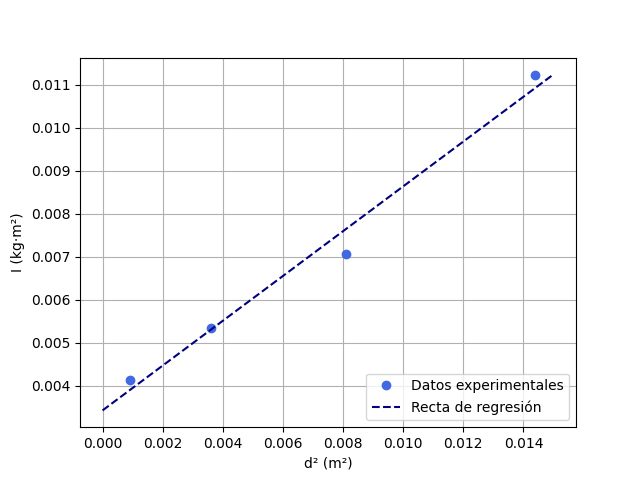
\includegraphics[width=0.85\linewidth]{Images/regSteiner1.png}
    \caption{Datos experimentales y regresión lineal del disco}
\end{figure}

A partir de los datos obtenidos en el ajuste podemos calcular el valor experimental de la masa del disco:

\begin{equation}
    m = 0.521 \pm 0.048 \; kg
\end{equation}

Si comparamos este valor con el medido directamente $(381,39 \;g)$ con la balanza podemos ver una clara diferencia. Esta diferencia puede tener explicaciones muy diversas, podría deberse a algún fallo experimental, a la falta de precisión en el ajuste que nos habría otorgado una regresión ponderada o a fallos en el cálculo. No obstante, el motivo que creemos que es culpable de la discordancia entre los valores es la falta de homogeneidad en los cuerpos. Siendo más concretos, cuando aplicamos el teorema de Steiner para hacer el ajuste estamos suponiendo que los cuerpos son ideales, homogéneos y con densidad constante. Este no es para nada nuestro caso, el disco se encontraba perforado y no se trataba de un disco ideal, cualquier heterogeneidad en su composición podría haber provocado esta diferencia.

\subsubsection{Barra rígida}

En el siguiente apartado vamos a tratar de verificar el teorema de Steiner en otro cuerpo diferente, una barra rígida de $65,7 \; cm$ de longitud y $0,12143 \; kg$ de masa. Como explicaremos en la metodología vamos a tomar medidas para 10 valores de $d$, en concreto tomamos solo 5 medidas del semiperíodo para cada valor de la distancia por problemas con el material.Los valores de $d$ para los que tomamos medidas con su incertidumbre son:

\begin{equation}
    d = n\cdot 1,0 \pm 0,1 \; cm \quad n = 1,2,3,...,10
\end{equation}

En las siguientes tablas representaremos los datos experimentales medidos en el laboratorio:








\section{Conclusiones}


\end{document}